\documentclass[10pt,a4paper]{article}
\usepackage[a4paper]{geometry}
\usepackage{amsmath}
\usepackage{amsfonts}
\usepackage{amssymb}

% Pretty figures
\usepackage{graphicx}

% Include paths.
\makeatletter
\makeatother
\graphicspath{
    {./}
}

\author{
    Ruben Taelman \\
    Sander Demeester \\
    Jens Rammant \\
    Eddy Van Den Heuvel \\
    Thomas Mortier \\
    Kevin Stobbelaar \\
    Felix Van der Jeugt
}

\title{
    Implementation Plan \\
    Avank Bebras
}

\setlength{\parskip}{12pt}
\setlength{\parindent}{0pt}

\begin{document}

\begin{section}{Subsystems}
	\begin{subsection}{Overview}
		These are the subsystems we will use in relation to each other. There is also an
		estimated percentage in each subsystem for how much work each subsystem will
		require.
		\begin{figure}[!h]
		  \centering
			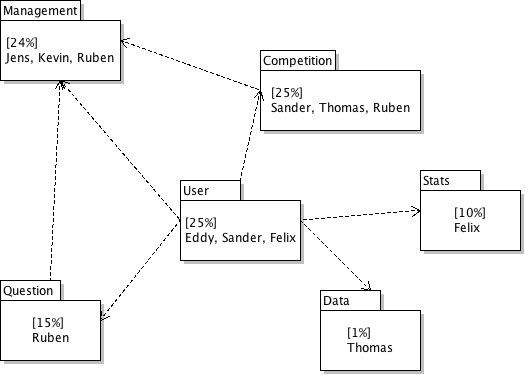
\includegraphics[width=1\textwidth]{../class_diagrams/subsystems.png}
		  \caption{Subsystems}
		  \label{subsystems}
		\end{figure}
	\end{subsection}
	
	\begin{subsection}{Contracts}
		% Hier moeten alle contracten tussen de subsystemen komen
		\begin{subsubsection}{Contract Competition-User}
	\begin{tabular}{l l l }
	  Client Class & Server Class & Explanation\\ \hline
	  Organizer & CompetitionManager & Competitions each User.\\
	  Organizer & Competition & Open, Start, Join and Finish a competition\\
	  Organizer & Competition & get the CompetitionUserState for a certain pupil\\
	  Organizer & CompetitionUserState & add grace time for a user\\
	\end{tabular}
\end{subsubsection}
		\begin{subsubsection}{Contract Question-Competition}
	\begin{tabular}{l l l }
	  Client Class & Server Class & Explanation\\ \hline
	  Competition & QuestionFeedback & gives feedback for a set of Answers\\
	\end{tabular}
\end{subsubsection}
		\begin{subsubsection}{Contract Question-User}
	\begin{tabular}{l l l }
	  Client Class & Server Class & Explanation\\ \hline
	  TODO & Question & define new questions\\
	  TODO & Server & define new servers\\
	\end{tabular}
\end{subsubsection}
		\begin{subsubsection}{Contract Database-User}
	\begin{tabular}{l l l }
	  Client Class & Server Class & Explanation\\ \hline
	  AuthenticationManager & TODO & Retrieve login data\\
	\end{tabular}
\end{subsubsection}
        	\begin{subsubsection}{Contract Statistics-User}
	\begin{tabular}{l l l }
	  Client Class & Server Class & Explanation\\ \hline
	  User & Statistics & Show statistics page.
	\end{tabular}
\end{subsubsection}

		\begin{subsubsection}{Contract Data-User}
	\begin{tabular}{l l l }
	  Client Class & Server Class & Explanation\\ \hline
	  Admin & TODO & Manage homepage links\\
		Admin & DataHandler & Manage Grades\\
		Admin & DataHandler & Manage Difficulties\\
		Admin & TODO & Manage FAQ
	\end{tabular}
\end{subsubsection}
        	\begin{subsubsection}{Contract Management-User}
	\begin{tabular}{l l l }
	    Client Class & Server Class & Explanation\\ \hline
        SuperUser & UserManager & List and manipulate pupils. \\
        Teacher & TODO & List and manipulate classgroups. \\
        Teacher & TODO & List and manipulate ongoing competitions.
	\end{tabular}
\end{subsubsection}

		\begin{subsubsection}{Contract Database-Management}
	\begin{tabular}{l l l }
	Client class & Server Class & Explanation \\ \hline
	QuestionManager & DatabaseManager & Create, read, update and delete questions \\
	CompetitionManager & DatabaseManager & Create, read, update and delete competitions \\
	UserManager & DatabaseManager & Create, read, update and delete users 
	\end{tabular}
\end{subsubsection}
	\end{subsection}
	
	% Hier moeten de subsystemen komen
	\begin{subsection}{SUBSYSTEM NAME}
	\textbf{Estimated amount of work: 24\%} \\
	\textbf{Responsible team member:} Jens, Kevin, Ruben \\
	\textbf{Class Diagram:} \\
	
	\begin{figure}[!h]
	    \centering
			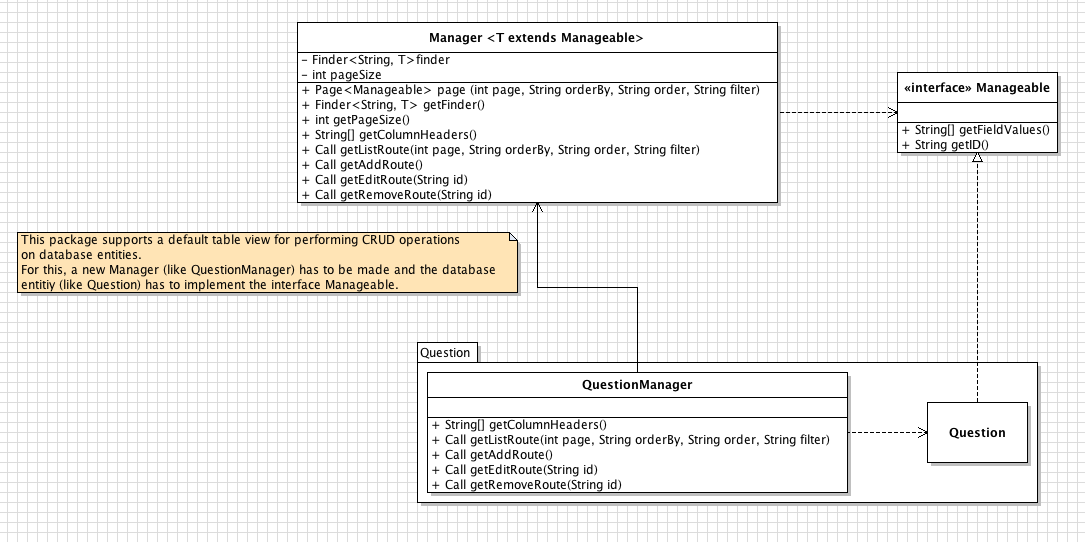
\includegraphics[width=1\textwidth]{../class_diagrams/management.png}
	    \caption{Subsystem Management}
	    \label{subsystem_management}
	\end{figure}

	\textbf{Remarks:} \\

\end{subsection}
	\begin{subsection}{Database}
	\textbf{Estimated amount of work:} 10\% \\
	\textbf{Responsible team member:} Jens, Kevin, Ruben \\
	\textbf{Class Diagram:} \\
	
	\begin{figure}[!h]
	  \centering
		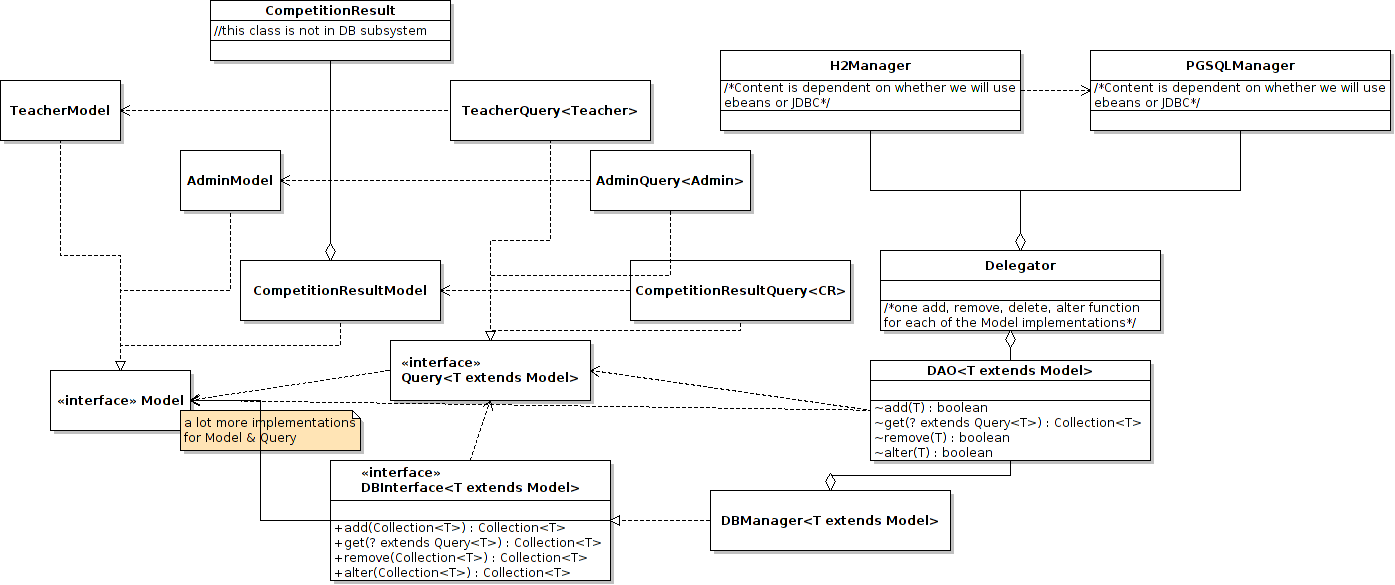
\includegraphics[width=1\textwidth]{../class_diagrams/database.png}
	  \caption{Subsystem Database}
	  \label{subsystem_database}
	\end{figure}
	
	\textbf{Remarks:} \\
	
\end{subsection}
	\begin{subsection}{Competition}
	\textbf{Estimated amount of work:} 25\% \\
	\textbf{Responsible team members:} Sander, Thomas, Ruben \\
	\textbf{Class Diagram:} \\
	
	\begin{figure}[h]
	  \centering
		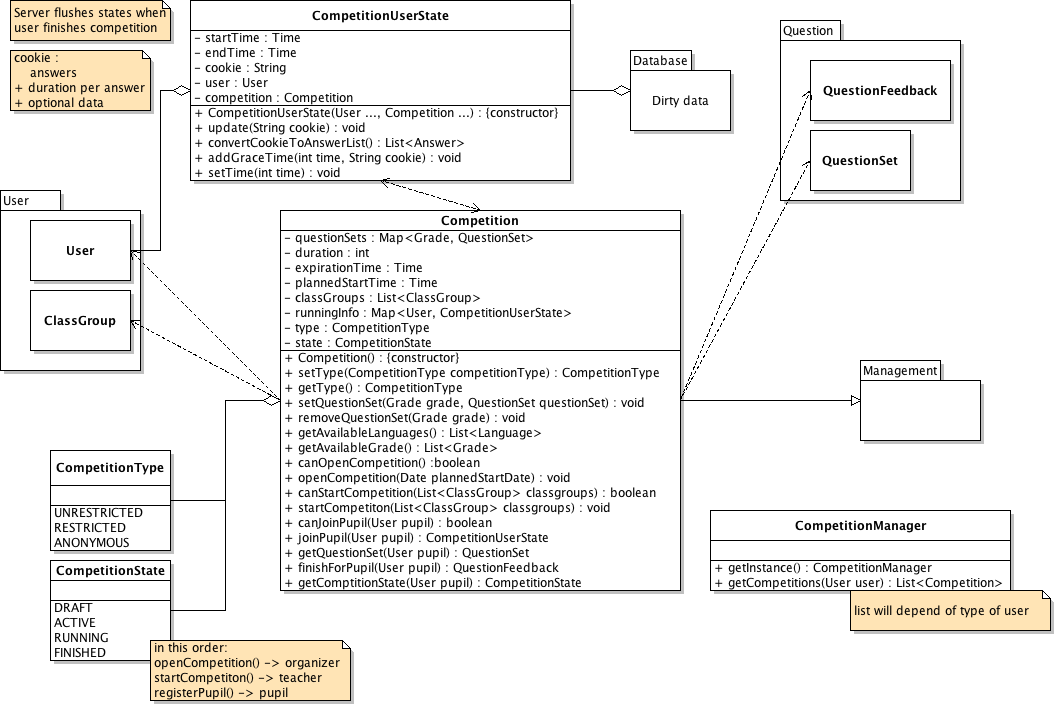
\includegraphics[width=1\textwidth]{../class_diagrams/competition.png}
	  \caption{Subsystem Competition}
	  \label{subsystem_competition}
	\end{figure}
	
\end{subsection}
	\begin{subsection}{Question}
	\textbf{Estimated amount of work:} 5\% \\
	\textbf{Responsible team member:} Ruben \\
	\textbf{Class Diagram:} \\
	
	\begin{figure}[!h]
	  \centering
		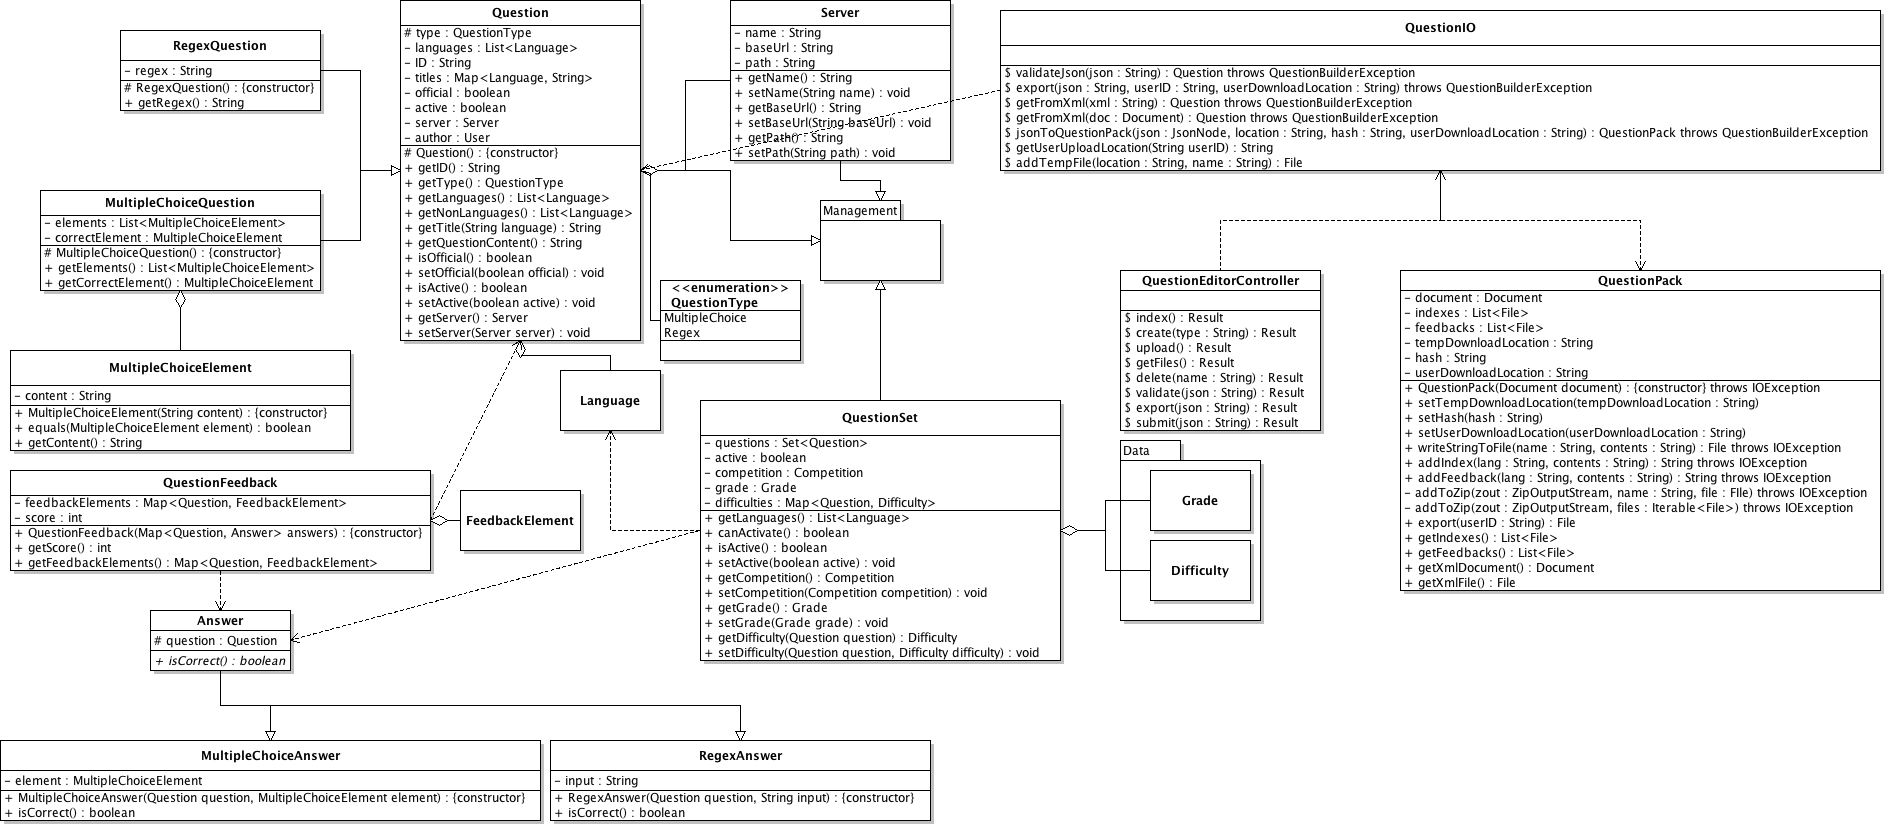
\includegraphics[width=1\textwidth]{../class_diagrams/question.png}
	  \caption{Subsystem Question}
	  \label{subsystem_question}
	\end{figure}
	
\end{subsection}
	\begin{section}{Pupil}
	When the student logins in he will be redirected to his dashboard where he will find information about his current status in the system. He will be able to see
	\begin{itemize}
	\item His current class (the class he is associated with).
	\item The previous competitions he took part in.
	\item List of competitions where he/she can participate in.
	\item A view to his personal statistics.
	\end{itemize}
	
\section*{Use-cases for Pupil}
\subsection*{Change password}
\subsubsection*{Main Success Scenario}
Actors: Student that is loged in.
\begin{itemize}
\item Step 1. Click on "change-password"
\item Step 2. User should be taking to a web-form to reset password
\item Step 3. Enter current password and email addres that is used for registering the account
\item Step 4. Enter in new password
\item Step 5. The user pressed submit
\item Step 6. The user should recieve an email that contains a activtion link for his new password.
\end{itemize}
\subsubsection*{Extentions}
\subsubsection*{Pre-conditions}
\begin{itemize}
\item The student should be logged in. 
\end{itemize}
\subsubsection*{Post-conditions}
\begin{itemize}
\item The user's password should be changed.
\end{itemize}
\subsubsection*{Triggers}
\begin{itemize}
\item The student clicked on "change password"
\end{itemize}
	
	\begin{subsection}{Statistics}
	\textbf{Estimated amount of work:} 10\% \\
	\textbf{Responsible team member:} Felix \\
	\textbf{Class Diagram:} \\
	
	\begin{figure}[!h]
	  \centering
		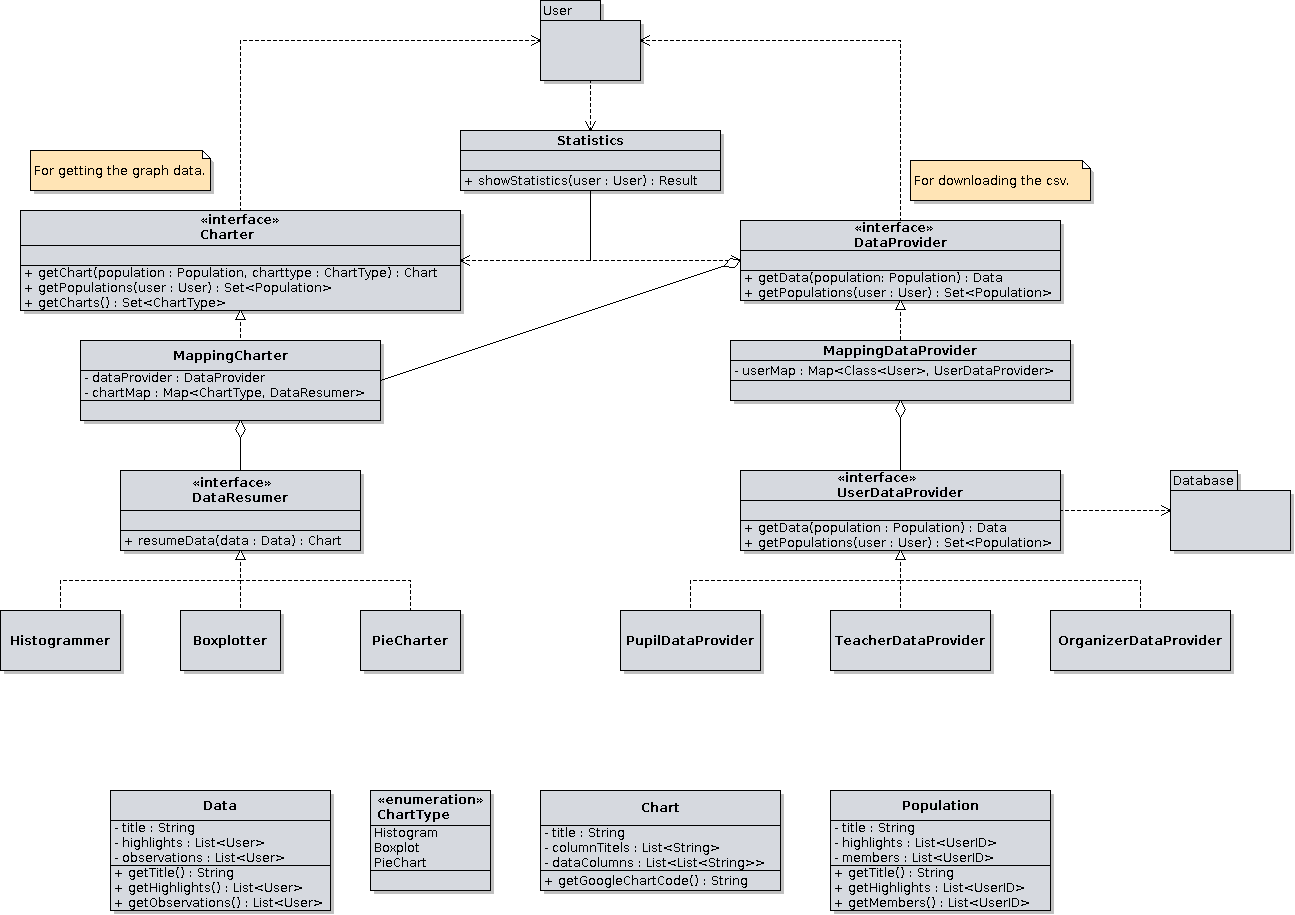
\includegraphics[width=1\textwidth]{../class_diagrams/statistics.png}
	  \caption{Subsystem Statistics}
	  \label{subsystem_question}
	\end{figure}
	
	\textbf{Remarks:} \\
	
\end{subsection}

	%\begin{subsection}{Data}
	\textbf{Estimated amount of work:} 1\% \\
	\textbf{Responsible team members:} Thomas\\
	\textbf{Class Diagram:} \\
	
	\begin{figure}[!h]
	  \centering
		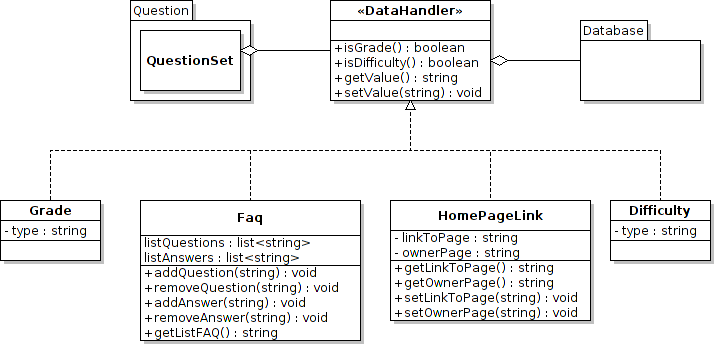
\includegraphics[width=1\textwidth]{../class_diagrams/data.png}
	  \caption{Subsystem Data}
	  \label{subsystem_data}
	\end{figure}

\end{subsection}

	
\end{section}	

\begin{section}{Implementation}
	% Dit moeten we nog bespreken
	The course of the implementation of each subsystem:
	\begin{itemize}
		\item Database:
		\begin{itemize}
			\item blablabla...
		\end{itemize}
  		\item Management:
  		\item User:
  		\item Question:
  		\item Competition:
  		\item Stats:
  		\item Data:
	\end{itemize}
\end{section}

% Use Cases nog invoegen?

\end{document}
